
\subsection*{First Calculations}
\subsubsection*{Assumptions}
Assumptions used:

\begin{enumerate}[label=\roman*.]
\item$\mu = 0$ (no slip boundary condition)
\item$\rho =constant$ (fluid is incompressible)
\item Control volume: $1\rightarrow 2\rightarrow3\rightarrow 4$ (uniform flow)
\item Immediately above and immediately below rotor blade: points 2,3 respectively
\item Induced velocity from rotor: $v_2=v_3=v_i$ (no velocity jump across disc)
\item Rotor blade assumed to be thin disc when in rotation
\item Pressure jump between sections 2 and 3 $(p2 \neq p3)$
\item $p_1=p_4=p_\infty$
\item Quasi-Steady flow
\item 1-D flow
\item Rotor treated as thin actuator disc
\item Quiescent flow outside of C.V.
\item $ Tip losses=0$   \\ 
 $\displaystyle{T.L.F=B=1-\frac{1.386\lambda_i}{N_b}}$   \\
 where $\displaystyle{\lambda_i=\frac{v_i}{v_tip}=\frac{v_i}{\Omega R}}$ , $N_b$= number of rotor blades
\item $A1>>A4$ and $v1<<v4$
\end{enumerate}

\begin{figure}[h!]
\begin{center}
  \includegraphics[scale=1]{Pictures/part1_fig1.png}
  % FOR OVERLEAF  \includegraphics[scale=1]{Romi/Pictures/part1_fig1.png}
  \caption{Control surfaces in controlled volume and x-y coordinate system set for 1 rotor where $T = thrust$ and $F_g= gravitational force of blade$ (replace sketch?)}
    \label{fig:romi_part1_fig1}
\end{center}
\end{figure}
\FloatBarrier
*Let CS = CSI + CSIII + ....... (Lumped CS)

\subsubsection*{Conservation of mass}
Using the conservation of mass, the mass flow rate through the boundary surfaces 1 and 4 is:
\begin{equation}
\frac{dM}{dt}\bigg|_s= \dot{m}_4 - \dot{m}_1 = 
\frac{\delta}{\delta x} \iiint\limits_{CV}\rho dV +\iint\limits_{CS} \rho  \overrightarrow{v}d \overrightarrow{A} 
\end{equation}

From assumption (ix): Quasi-steady, so $\iiint\limits_{CV}\rho dV = 0$
Expression (1) now becomes 
$$ \frac{dM}{dt}\bigg|_s= \dot{m}_4 - \dot{m}_1 =0 $$

Since the mass flow rates across all boundaries are equivalent:
\begin{align}
\dot{m}_1 = \dot{m}_2 &= \dot{m}_3 = \dot{m}_4 \\
\dot{m}_i &= \rho A_i\ v_i
\end{align}

\subsubsection*{Conservation of momentum}
The momentum equation for the inertial volume is:
\begin{equation}
\sum F\big|_s= 
\frac{\delta}{\delta x} \iiint\limits_{CV}\rho \overrightarrow{v} dV +\iint\limits_{CS} \overrightarrow{v}\rho  \overrightarrow{v}d \overrightarrow{A} 
\end{equation}
Momentum components in x,y directions, see fig X for system sketch: $ \overrightarrow{F}_y =0  $ (no forces in y direction)
\begin{align}
\sum F = T - \frac{W}{2} = 0\\
-R_x = T = \frac{W}{2} =  \dot{m}_4 \dot{v}_4 -  \dot{m}_1 \dot{v}_1
\end{align}
From assumption (xiv)
\begin{equation}
T = \frac{W}{2} =  \dot{m}_4 \dot{v}_4
\end{equation}
\subsubsection*{Conservation of energy}
\begin{equation}
\dot{Q} - \dot{W} =
\frac{dE}{dt}\bigg|_s= \dot{m}_4 - \dot{m}_1 = 
\frac{\delta}{\delta x} \iiint\limits_{CV}e \rho dV +\iint\limits_{CS} e\rho  \overrightarrow{v}d \overrightarrow{A} 
\end{equation}

where $e=u+\frac{P}{\rho}+\frac{v^2}{2}+gz $ and $\dot{W}=\dot{W}_{Shaft}+\dot{W}_{normal \, stress}+\dot{W}_{others}$
From assumption (ix) and since the system is isothermal we get:

Equation ( 3 ) now becomes:
\begin{equation}
P_{i, \text {ideal}}=T v_{i}=\iint_{c s}\left(u+\frac{p}{\rho}+\frac{v^{2}}{2}+g z\right) \rho \vec{v} \cdot d \vec{A} \quad(\text { from } \operatorname{cs} 1 \vec{D} 4)
\end{equation}

From assumption (i)  inviscid and incompressible flow: $u=0$ $*$ From assumption (viii) $ p_{1}=p_{4}=p_{\infty}$ \\
From assumption (xi) height is negligible in an actuator disc $ z_{4}-z_{1}=0$
Equation ( 3.1 ) can be re-written as:
\begin{align}
P_{i, \text {ideal}}=T v_{i}=&\left[\frac{P_{4}}{\rho}+\frac{v_{4}^{2} \dot{m}_{4}}{2}+g z_{4}\right]-\left[\frac{P_{1}}{\rho}+\frac{v_{1}^{2} m_{1}}{2}+g z_{1}\right] \\
& T v_{i}=\frac{1}{2} v_{4}^{2} \dot{m}_{4}-\frac{1}{2} v_{1}^{2} \dot{m}_{1}
\end{align}
From assumption $(x i v)  m i_{1} \dot{v}_{1}=0,$ the above equation can be re-written as:
\begin{equation}
P_{i, \text {ideal}}=T v_{i}=\frac{1}{2} v_{4}^{2} \dot{m}_{4}
\end{equation}

Plugging equation (2.2) into (3.2):

\begin{equation}
P_{i, i d e a l}=T v_{i}=\frac{1}{2} v_{4}^{2} m_{4} \\
P_{i, i d e a l}=m_{4} v_{4} v_{i}=\frac{1}{2} v_{4}^{2} m_{4} \\
 v_{i}=\frac{v_{4}}{2} \text { or } v_{4}=2 v_{i}
\end{equation}

Using Bernoulli's Equation for Frictionless, Incompressible and Steady Flow:
Basic equation: $$p_{1}+\frac{\rho v_{1}^{2}}{2}+\rho g z_{1}=p_{2}+\frac{\rho v_{2}^{2}}{2}+\rho g z_{2}$$
From assumption (viii) $ p_{1}=p_{4}=p_{\infty}$\\
At $\mathrm{p}_{1}$  $\mathrm{p}_{2}$

\begin{align}
p_{1}+\frac{\rho v_{1}^{2}}{2}+\rho g z_{1}&=p_{2}+\frac{\rho v_{2}^{2}}{2}+\rho g z_{2} \\
p_{\infty}&=p_{2}+\frac{\rho v_{i}^{2}}{2} \\
p_{\infty}&=p_{2}+\frac{\rho v_{i}^{2}}{2}
\end{align}

At $\mathrm{p}_{3}$  $\mathrm{p}_{4}$ :
\begin{align}
p_{3}+\frac{\rho v_{3}^{2}}{2}+\rho g z_{3} &=p_{4}+\frac{\rho v_{4}^{2}}{2}+\rho g z_{4} \\
p_{3}+\frac{\rho v_{i}^{2}}{2} &=p_{\infty}+\frac{\rho v_{4}^{2}}{2} \\
p_{3}+\frac{\rho v_{i}^{2}}{2}-\frac{\rho v_{4}^{2}}{2}&=p_{\infty}
\end{align}

Let equations $(4.1)=(4.2)$

\begin{align}
p_{3}+\frac{\rho v_{i}^{2}}{2}-\frac{\rho v_{4}^{2}}{2}=p_{2}+\frac{\rho v_{i}^{2}}{2} \\
p_{3}-p_{2}=\frac{\rho v_{4}^{2}}{2}+\left(\frac{\rho v_{i}^{2}}{2}-\frac{\rho v_{i}^{2}}{2}\right) \\
\Delta p=p_{3}-p_{2}=\frac{\rho v_{4}^{2}}{2} \\
\text { Thrust }=T=A \Delta p
\end{align}

Plugging in (4.3) into (4.4)
\begin{equation}
T=A \Delta p=A\left(\frac{\rho v_{4}^{2}}{2}\right)
\end{equation}


plugging in (3.3) into (4.5):
\begin{equation}
T=A \Delta p=A\left(\frac{\rho\left(2 v_{i}\right)^{2}}{2}\right)
\end{equation}

Solving for $v_i$ yields:
\begin{equation}
v_{i}=\sqrt{\frac{T}{2 \rho A}}
\end{equation}
The ideal induced power Pijdenl (in kw) of each rotor by using the momentum theory is:
Plugging in equation (4.6) into (3.2) \\
\begin{align}
P_{i, ideal}= Tv_i = T\left(\sqrt{\frac{T}{2 \rho A}}\right) = T\left(\sqrt{\frac{T}{2 \rho \pi R^2}}\right)
\end{align}




(ADD IN VALUES)










